\subsubsection{Traversing the hit list by e-value}

The candidate orthologs are sorted by the e-value of their respective HMM
search. By doing so, it is assured that the most relevant candidate is assigned
a transcript. This avoids a ``first come, first serve'' scenario in which a
candidate with a high e-value gets assigned a transcript that is then no longer
available for a candidate with a lower e-value.

\subsubsection{Removing hits from the candidate list eliminates redundancy}

In order to avoid redundant assignment, i.e., a single transcript being assigned
to multiple ortholog groups or vice versa, candidate pairs that have been
verified are removed from the list of candidates. 

\begin{figure}[ht]
	\begin{center}
		%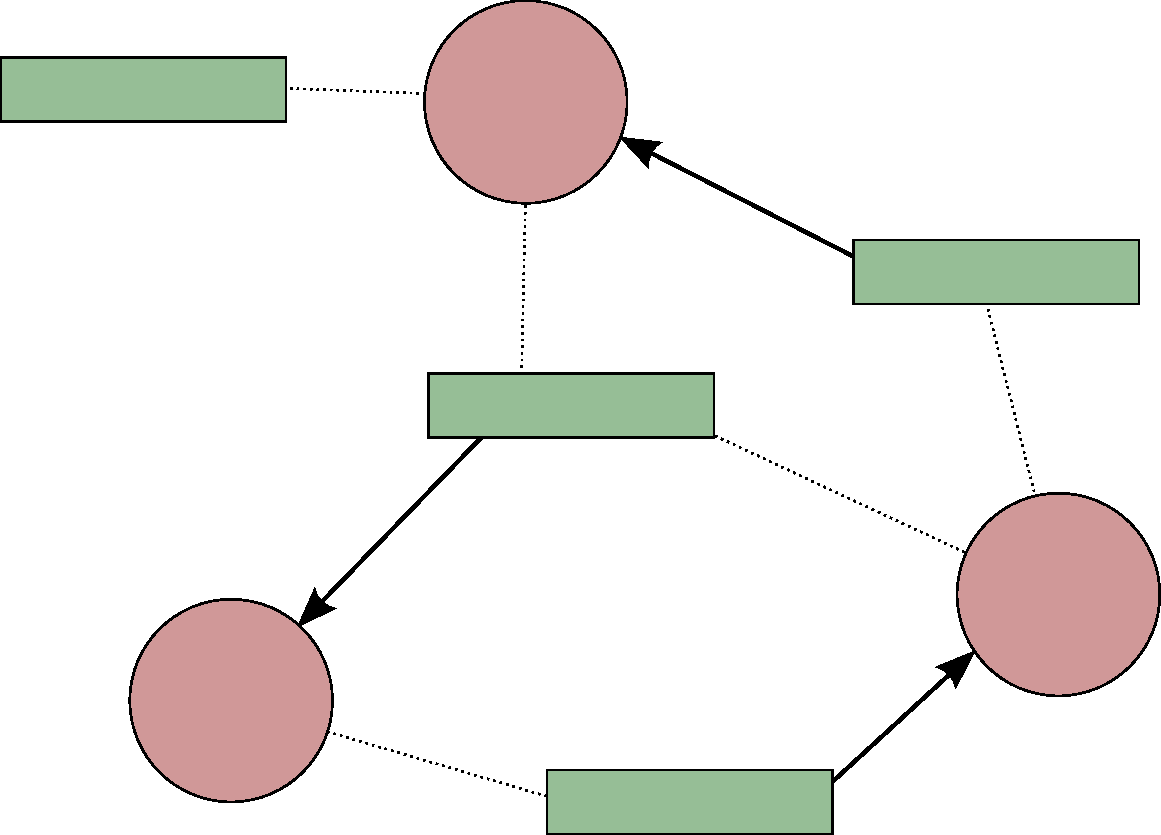
\includegraphics[width=0.8\textwidth]{img/orthograph_graph.pdf}
	\end{center}
	\caption{A two-dimensional graph. The ortholog groups (OG) are connected to the
	candidate hit transcripts by the e-value of the HMM search. Traversing the graph
	by e-value and assigning the transcripts to the OG with the best
	hit results in transcript 2 being assigned to OG A, transcript 3 to OG B and
	transcript 4 to OG C. Transcript 1 remains unassigned because the HMM search
	e-value for OG A is higher than the e-value for transcript 2.}
	\label{fig:graph}
\end{figure}
